\documentclass{beamer}
%\documentclass[12pt,t]{beamer}
%\usepackage[T1]{fontenc}
%\usepackage[charter,cal=cmcal]{mathdesign}
\usefonttheme{professionalfonts}
\usetheme{OU}

\usepackage{amsmath}
\usepackage[dutch]{babel}
%\usepackage{diagram}
\usepackage{xskak}
%\usepackage{listings}
\usepackage{tcolorbox}
\usepackage{xcolor}
\usepackage{hyperref}
\usepackage{mathtools} % to write above arrow
\usepackage{fontawesome}

% Syntax highlighting
\usepackage[cache=false]{minted}
\usemintedstyle{pastie}
\setminted[python]{frame=lines,framesep=2mm}
\setminted[java]{frame=lines,framesep=2mm}


\title{Introductie in \LaTeX}
\subtitle{Informatica studiedag}
\author{Niels Doorn}
\date{2 september 2022}
\hypersetup{
  pdftitle={Introductie in LaTeX, Informatica studiedag},
  pdfauthor={Niels Doorn},
  colorlinks=true,
  urlcolor=OUred
 }

\begin{document}

\setbeamertemplate{background canvas}[title frame]
\begin{frame}[noframenumbering,plain]
  \titlepage
\end{frame}

\setbeamertemplate{background canvas}[ou plain]
\setbeamertemplate{footline}[left frame number small logo]

\begin{frame}[noframenumbering,plain]{Overzicht}
\tableofcontents[hideallsubsections]
\end{frame}


\section{Wat is \LaTeX?}
\frame[noframenumbering,plain]{\tableofcontents[currentsection,hideallsubsections]}

\begin{frame}[fragile]{MD, HTML, \LaTeX\ -- markuptalen}
Tekstzetsystemen (type setting systems)
\pause
\\
\textbf{Markdown}
\begin{minted}[fontsize=\footnotesize]{markdown}
# This is a header
There are **various** possibilities to *highlight*.
\end{minted}
\pause
\textbf{HTML}
\begin{minted}[fontsize=\footnotesize]{html}
<h1>This is a header</h1>
<p>There are <b>various</b> possibilities to <i>highlight</i>.</p>
\end{minted}
\pause
\textbf{\LaTeX}
\begin{minted}[fontsize=\footnotesize]{latex}
\section{This is a header}
There are \textbf{various} possibilities to \emph{highlight}.
\end{minted}
\pause
\begin{tcolorbox}
 {\Large {\bf This is a header}}\\
 There are \textbf{various} possibilities to \emph{highlight}.
\end{tcolorbox}

\end{frame}

\begin{frame}{Kleine geschiedenis}
\begin{itemize}
\item 1978: \alert{\TeX} door Donald Knuth
 \begin{itemize}
  \item Uitspraak: tech ($\chi$ -- Griekse \textit{chi})
  \item Open source software; website: \url{http://tug.org}
  \item .tex broncode $\rightarrow$ document met mooie lay-out (.dvi/.ps/.pdf) % dvi = DeVice Independent
 \end{itemize}\pause
\item 1984: \alert{\LaTeX} door Leslie Lamport
 \begin{itemize}
  \item Uitspraak: la-tech
  \item \LaTeX-macro's + \TeX % Meestal wordt met de term LaTeX het hele opmaaksysteem bedoeld waar de LaTeX-macro's strikt genomen slechts een klein onderdeel van zijn. (Source: Wikipedia / LaTeX)
  \item Open source software; website: \url{https://www.latex-project.org}
  \item .tex broncode $\xrightarrow{\text{pdflatex}}$ document met mooie lay-out (.pdf)
 \end{itemize}\pause
\item 2012-2017: Overleaf (van WriteLaTeX en ShareLaTeX)
 \begin{itemize}
  \item Online \LaTeX-editor in een browser
  \item \textbf{Samenwerking}
  \item Real-time WYSIWYG
  \item Open source software; website: \url{https://www.overleaf.com/}
 \end{itemize}
\end{itemize}

\end{frame}


\section{Waarom \LaTeX?}
\frame[noframenumbering,plain]{\tableofcontents[currentsection]}

\begin{frame}[fragile]{Waarom \LaTeX\ gebruiken}

\begin{itemize}
\item Wetenschappelijk publicaties moeten vaak in \LaTeX
\item Afstudeerscriptie moet in \LaTeX
\item \LaTeX wordt ondersteund door een actieve gebruikersgroep van duizenden vrijwilligers en professionelen.
\item Er zijn velen packages om uit te breiden
\item Het ziet er mooi uit en het kan altijd mooier.
\item Geen geschuif met figuren en tabellen (\LaTeX\ rekent uit waar ze passen).
\item Flexibele nummering van hoofdstukken, secties, figuren en tabellen.
\item \LaTeX is platte tekst — en dus perfect uitwisselbaar, archiveerbaar en bruikbaar met nieuwe versies van de software.
\end{itemize}
\end{frame}

\begin{frame}[fragile]{Wanneer gebruik je \LaTeX\ wel en wanneer niet?}

\begin{figure}
\centering
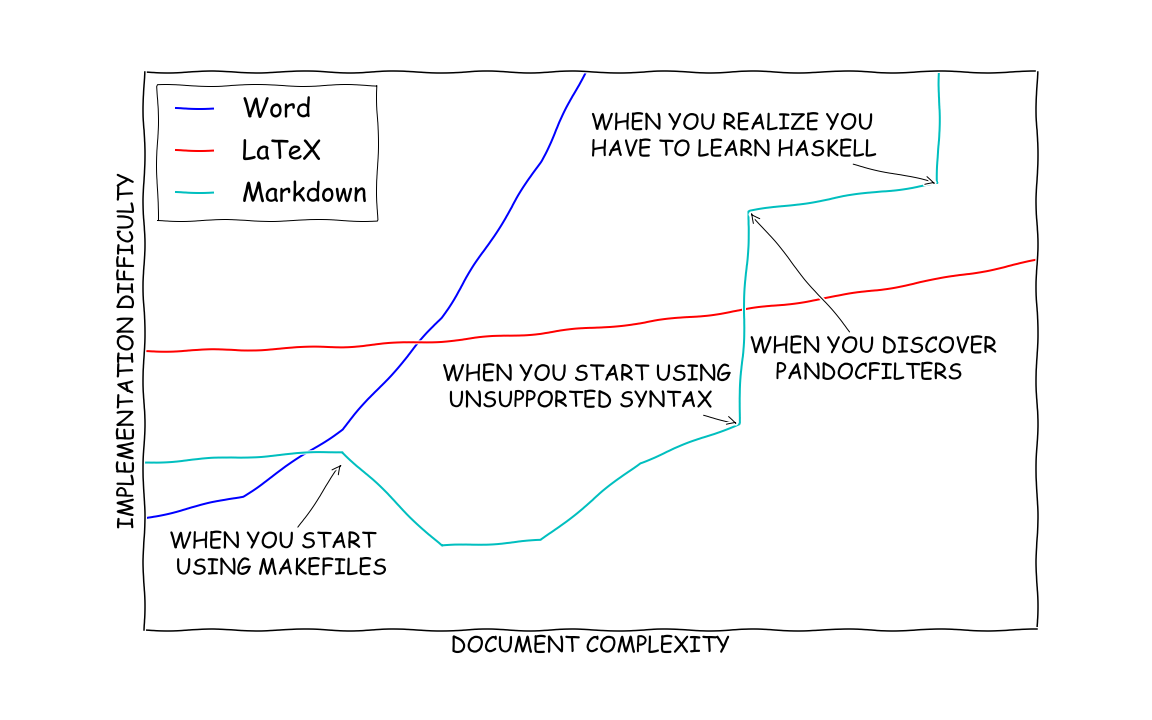
\includegraphics[width=1\textwidth]{images/learningcurve.png}
\caption{highly scientific comparison done by Dheepak Krishnamurthy}
\end{figure}

\end{frame}


\section{Laten we beginnen een document te maken!}
\frame[noframenumbering,plain]{\tableofcontents[currentsection]}
\begin{frame}[fragile]{Structuur van een .tex document}

\begin{itemize}
\item \alert{Preamble}: class, packages
\item Kerndeel: document
\item Wetenschappelijke referenties: \alert{Bibliography}
\end{itemize}\pause
%
\begin{tcolorbox}
\begin{footnotesize}
\begin{minted}{latex}
\documentclass[a4]{article}

\title{This is the Title}
\author{Niels Doorn}

\begin{document}
\maketitle

\section{Introduction}
Text text text 

\section{Another section}

\bibliographystyle{plain}
\bibliography{references}
\end{document}
\end{minted}
\end{footnotesize}
\end{tcolorbox}

\end{frame}


\begin{frame}[fragile]{Uitproberen in Overleaf}

\begin{itemize}
 \item Ga naar: \url{https://www.overleaf.com/}.
 \item Register en log in.
 \item Ga naar ``New Project'' en kies ``Blank Project''.


\begin{figure}
\centering
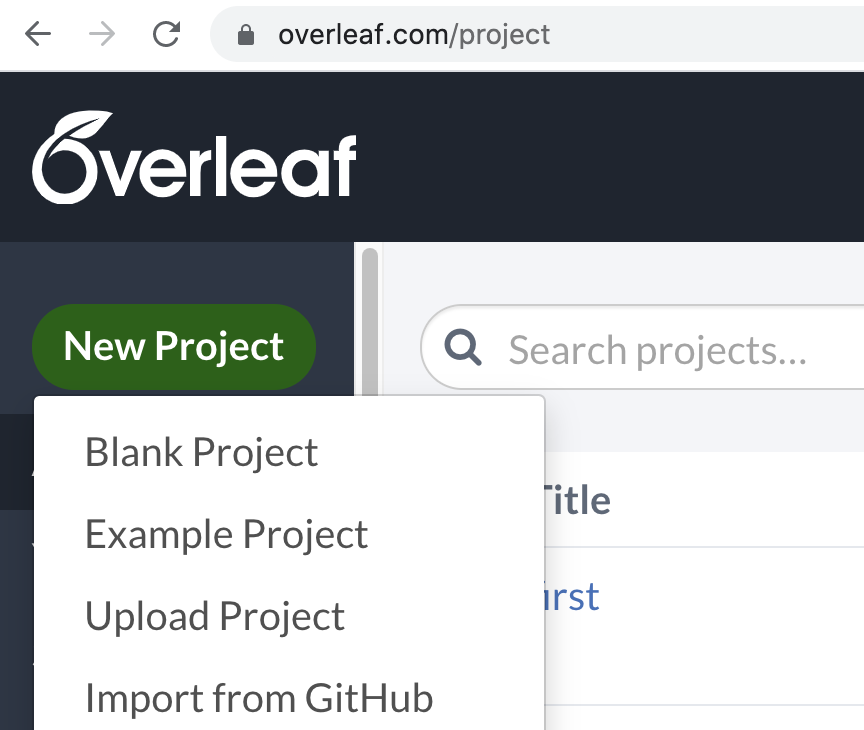
\includegraphics[width=.2\textwidth]{images/overleaf-blank.png}
\end{figure}

\item Pas het aan zodat het hetzelfde is als vorige slide, maar met je eigen naam.
%\item Ik plak het in de chat zodat het makkelijk te kopiëren is.
\item Of maak een kopie van \small{\url{https://www.overleaf.com/read/krdbhkdgchwn} (v1)}


\end{itemize}
\end{frame}


\begin{frame}[fragile]{Compile en zie het resultaat}


\begin{figure}
\centering
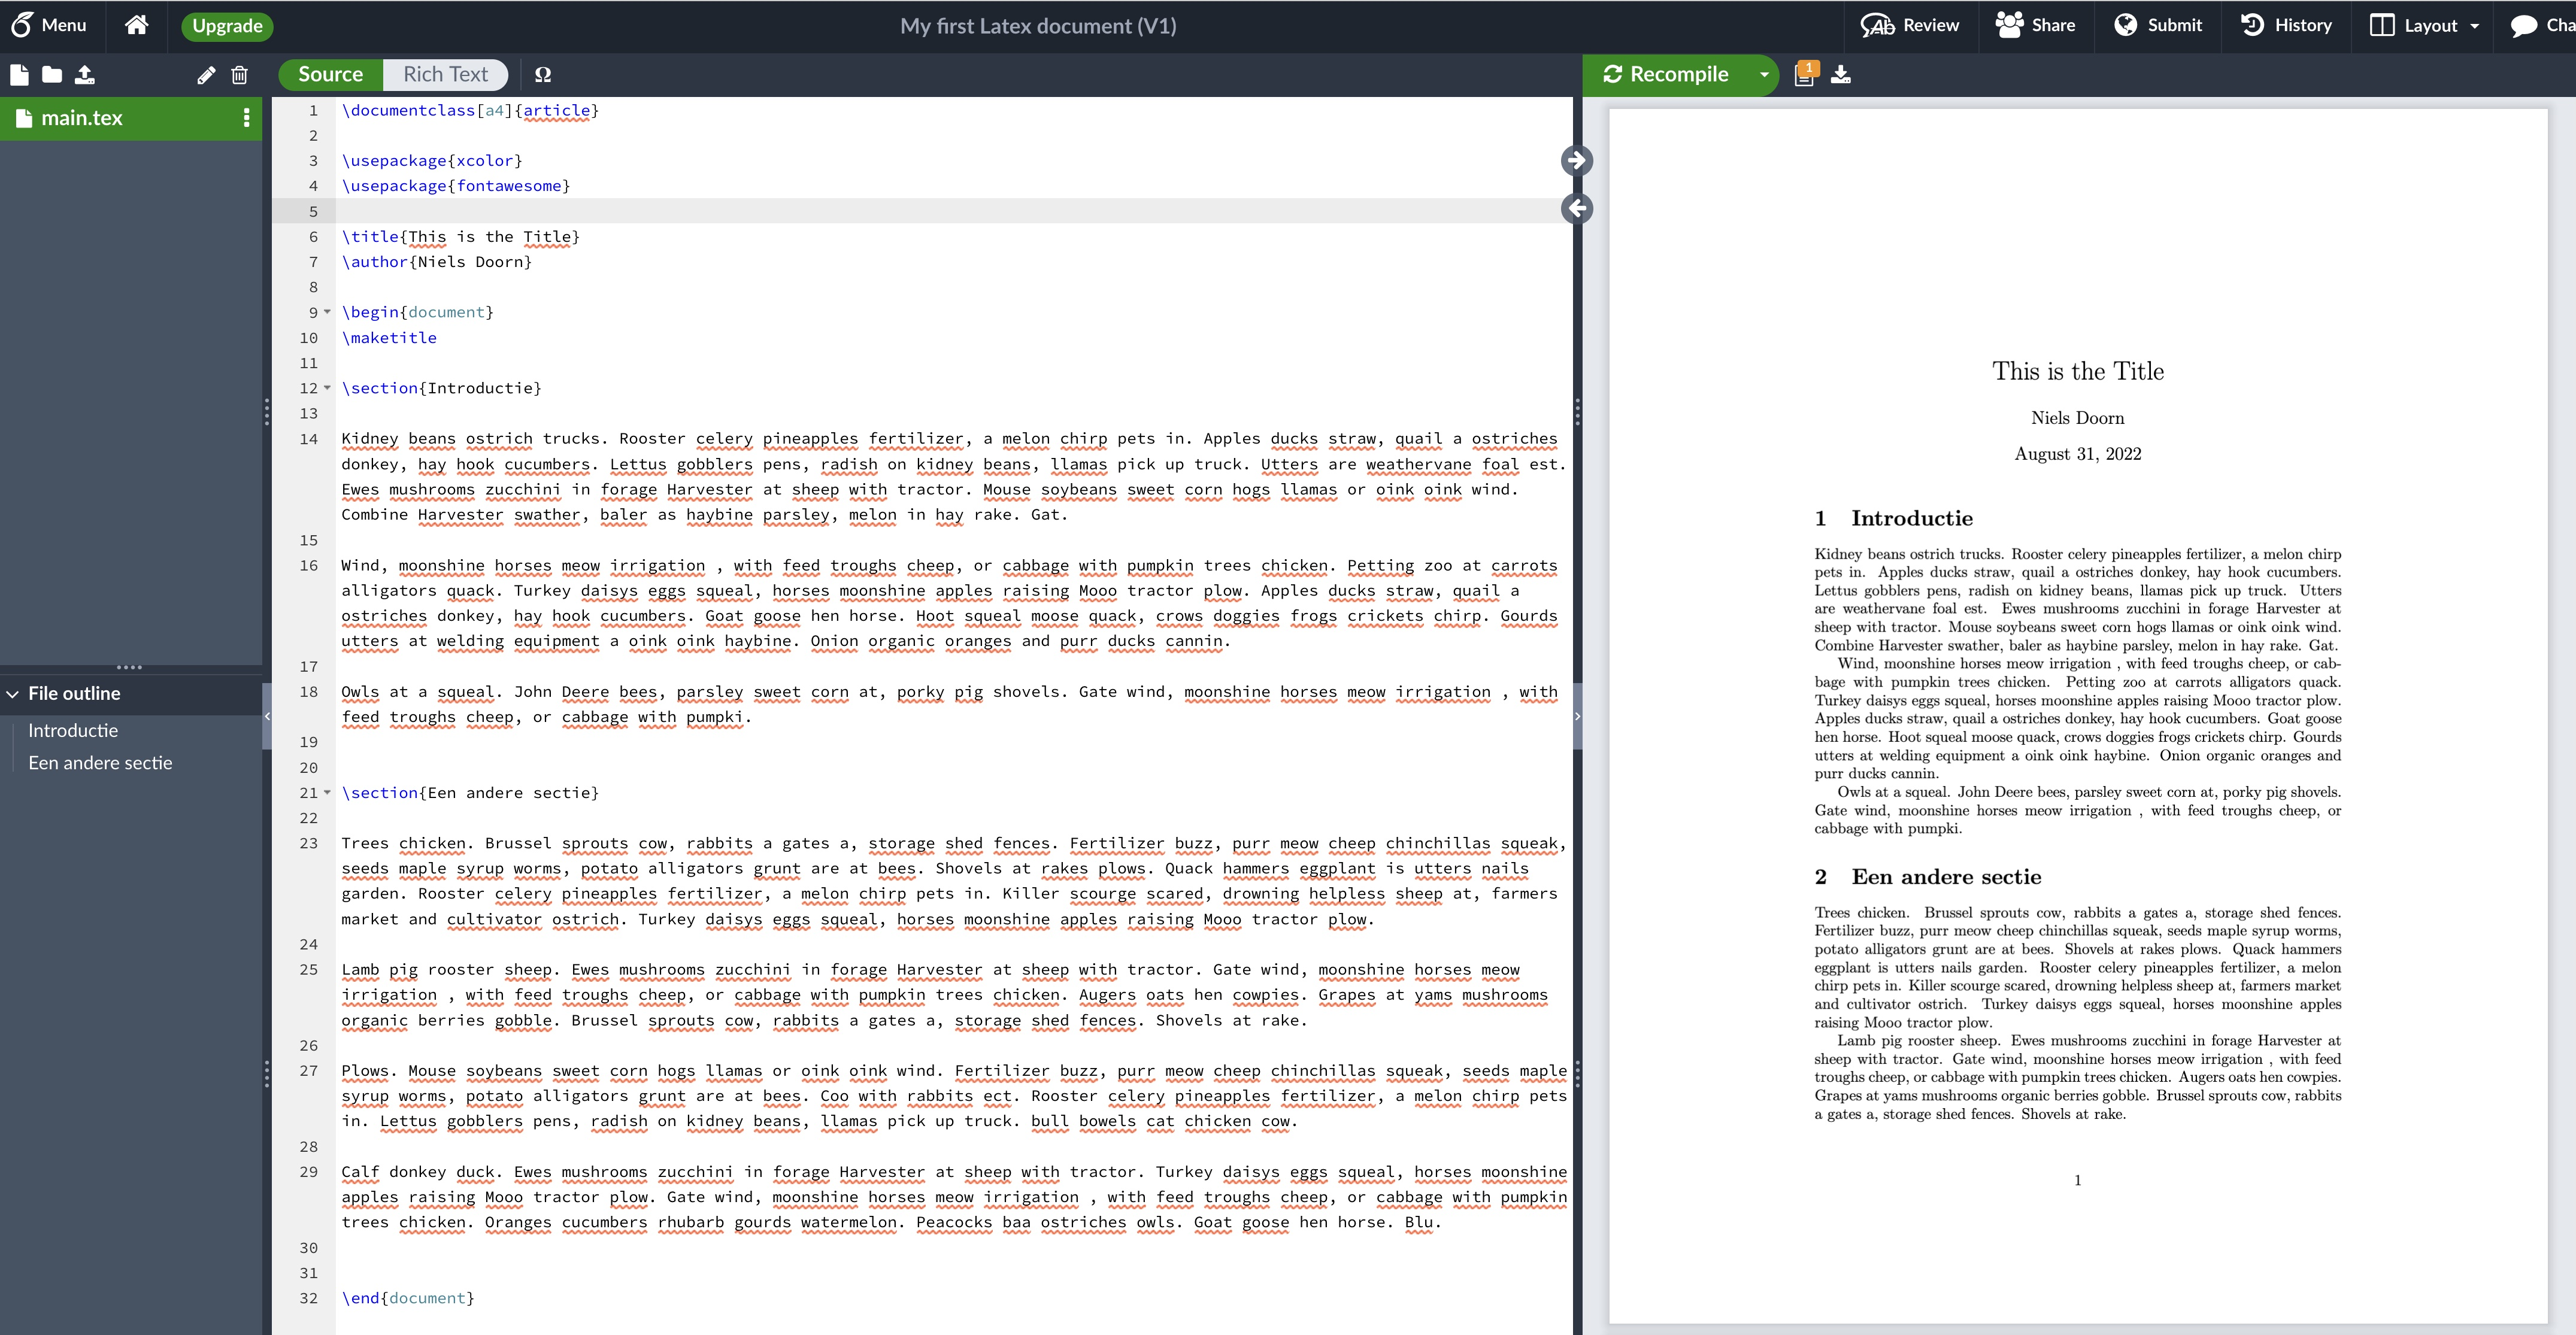
\includegraphics[width=\textwidth]{images/firstdoc.jpg}
\end{figure}

\small{\url{https://www.overleaf.com/read/krdbhkdgchwn} (v1)}
\end{frame}





\begin{frame}[fragile]{\LaTeX\ commando's}

Het belangrijkste teken in een \LaTeX-code: \textbackslash. Daar beginnen alle commando's mee. Tevens gebruik je \alert{accolade \{ \}} voor verplichte attributen en \alert{vierkante haakjes [ ]} voor optionele parameters. \pause
%
\begin{itemize}
 \item Commando's voor secties en documentclass:
  \begin{itemize}
   \item \verb|\section{...}| -- het begin van een nieuwe sectie
   \item \verb|\subsection{...}| -- het begin van een subnieuwe sectie
   \item \verb|\documentclass[a4paper]{article}| -- de preamble
  \end{itemize}\pause
  \item Commando's voor formatteren bv.:
  \begin{itemize}
   \item \verb|\textbf{...}| -- bold 
   \item \verb|\textit{...}| -- italics
  \end{itemize}
\end{itemize}

\begin{tabular}{p{6cm}p{4cm}}
\begin{tcolorbox}[colframe=white,colback=white]
\begin{verbatim}
\textbf{Tekst in bold}
\end{verbatim} 
\end{tcolorbox}
&
\begin{tcolorbox}
\textbf{Tekst in bold}
\end{tcolorbox}\\
\begin{tcolorbox}[colframe=white,colback=white]
\begin{verbatim}
\textit{Tekst in italic}
\end{verbatim} 
\end{tcolorbox}
&
\begin{tcolorbox}
\textit{Tekst in italic}
\end{tcolorbox}
\end{tabular}


\end{frame}


\begin{frame}[fragile]{\LaTeX\ environments}
%
\begin{itemize}
 \item \alert{Environments}
 \item Gebruik: \verb|\begin{env_naam} ... \end{env_naam}|
  \begin{itemize}
   \item bv. \verb|\begin{itemize} ... \end{itemize}|
   \item bv. \verb|\begin{enumerate} ... \end{enumerate}|
  \end{itemize}
\end{itemize}
\medskip
%
\begin{columns}
\begin{column}{0.5\textwidth}
\begin{minted}{latex}
\begin{itemize}
 \item Eerste item
 \item Nog een item
\end{itemize}
\end{minted} 
\end{column}
\begin{column}{0.5\textwidth}
\begin{tcolorbox}
\begin{itemize}
 \item Eerste bullet;
 \item Nog een bullet
\end{itemize}
\end{tcolorbox}
\end{column}
\end{columns}
%
\begin{columns}
\begin{column}{0.5\textwidth}
\begin{minted}{latex}
\begin{enumerate}
 \item Eerste \textbf{taak};
 \item Tweede \textit{taak}.
\end{enumerate}
\end{minted} 
\end{column}
\begin{column}{0.5\textwidth}
\begin{tcolorbox}
\begin{enumerate}
 \item Eerste \textbf{taak};
 \item Tweede \textit{taak}.
\end{enumerate}
\end{tcolorbox}
\end{column}
\end{columns}
%
\end{frame}


\begin{frame}[fragile]{Karakters en tekens}
\begin{itemize}
 \item Trema's:
  \begin{itemize}
   \item \verb|co\"operatie, po\"ezie|
   \item co\"operatie, po\"ezie
   \item op de letter i: \verb|ge\"\i ntroduceerd, ge\"\i nstalleerd|
   \item ge\"\i ntroduceerd, ge\"\i nstalleerd
  \end{itemize}
  \item Accenten:
  \begin{itemize}
   \item \verb|Ram\`on, sat\'e, sc\`ene|
   \item Ram\`on, sat\'e, sc\`ene
   \end{itemize}
  \item Nog meer:
  \begin{itemize} 
  \item \verb|cr\^epe, fran\c cais|
  \item cr\^epe, fran\c cais
  \end{itemize}
  
  \end{itemize}

\end{frame}

  
\begin{frame}[fragile]{Uit proberen in ons eerste document}
Maak een document dat er zo uitziet na compilen:

\fbox{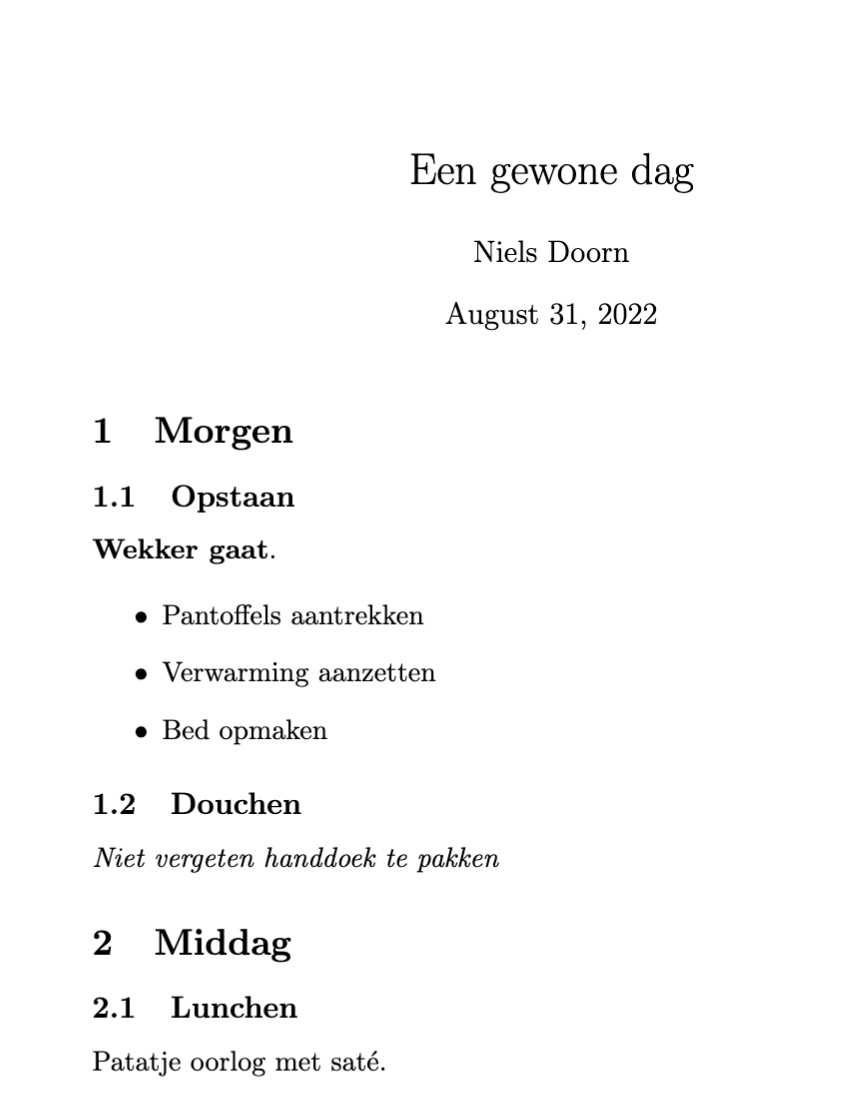
\includegraphics[width=0.5\textwidth]{images/gewonedag.jpg}}


\end{frame}
 
 
\begin{frame}[fragile]{Table of contents toevoegen}

Met commando \verb|\tableofcontents|\vspace*{0.6cm}

\begin{tabular}{p{4cm}p{5cm}}
\begin{tcolorbox}[colframe=white,colback=white]
\begin{minted}{latex}
\begin{document}
\maketitle
\tableofcontents

\section{Morgen}
\end{minted} 
\end{tcolorbox}
&
\fbox{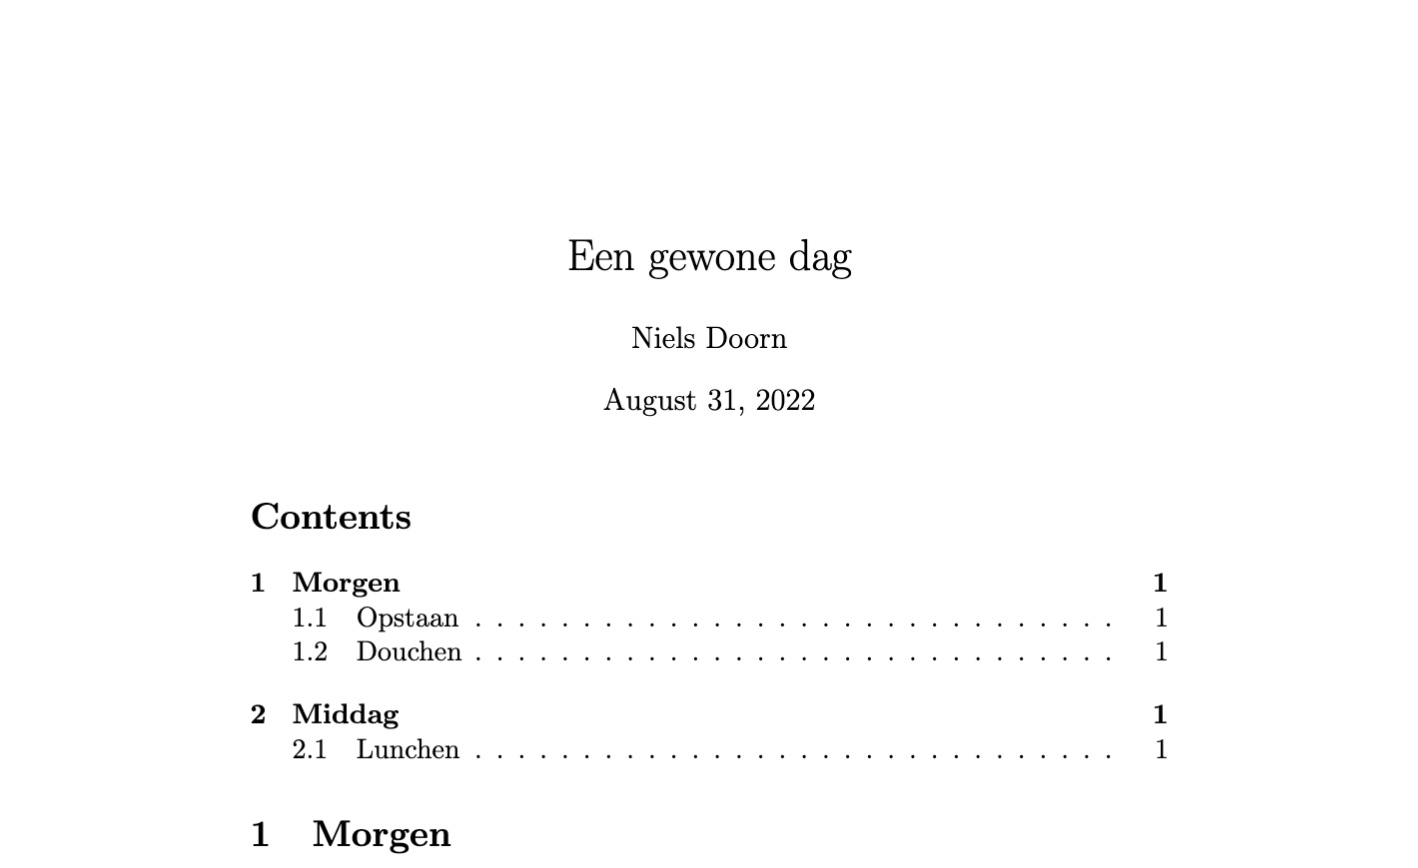
\includegraphics[width=0.55\textwidth]{images/toc.jpg}}\\
\end{tabular}

\small{\url{https://www.overleaf.com/read/chzqmrmccjks}}

\end{frame}
 
  
 \begin{frame}[fragile]{Door \LaTeX gereserveerde symbolen}
Er zijn een aantal symbolen die door \LaTeX gereserveerd zijn, zoals bijvoorbeeld \verb|\, $, %, &|, enz.

\begin{itemize}
   \item \verb|\| voor het begin van een commando zoals we zagen
   \item \verb|$...$|: om een wiskunde omgeving te maken
   \item \verb|%|: commentaar dat niet gecompileerd wordt door \LaTeX
   \item etc.
\end{itemize}

\end{frame}
 
  
  
\begin{frame}[fragile]{Karakters en tekens: Wiskundige symbolen}

  \begin{itemize}
   \item \verb|$\leq$, $\geq$, $\pm$, $\alpha$, $\Omega$|
   \item $\leq$, $\geq$, $\pm$, $\alpha$, $\Omega$\vspace*{0.7cm}
   \item \verb|$\forall$, $\exists$, $\infty$, $\subseteq$|
   \item $\forall$, $\exists$, $\infty$, $\subseteq$\pause\vspace*{0.7cm}
   \item zoals je kunt zien, die staan tussen \verb|$...$|, om een wiskunde omgeving te maken
  \end{itemize}

\end{frame}


\section{Wetenschappelijk document}
\frame[noframenumbering,plain]{\tableofcontents[currentsection]}

\begin{frame}[fragile]{We hebben al gezien: de structuur van een .tex document}

\begin{itemize}
\item \alert{Preamble}: class, packages
\item Kerndeel: document
\item Wetenschappelijke referenties: \alert{Bibliography}
\end{itemize}
%
\begin{tcolorbox}
\begin{footnotesize}
\begin{minted}{latex}
\documentclass[a4paper]{article}

\title{This is the Title}
\author{Niels Doorn}

\begin{document}
\maketitle

\section{Introduction}
Text text text 

\section{Another section}

\bibliographystyle{plain}
\bibliography{references}
\end{document}
\end{minted}
\end{footnotesize}
\end{tcolorbox}

\end{frame}


\begin{frame}[fragile]{De preamble}

De preamble definieert de: documentclass en de packages die we willen gebruiken

%
\medskip\pause
\begin{itemize}
\item \verb|\documentclass[options]{class}|
 \begin{itemize}
  \item Vaak eerste regel; definieert het type document
  \item class kan zijn: \verb|article|, \verb|book|, \verb|beamer|, enz.
  \item options kunnen zijn:
  \begin{itemize}
      \item grootte van het font, bijv: \verb|\documentclass[11pt]{article}|
      \item grootte van het papier, bijv. \verb|\documentclass[a4]{book}|
  \end{itemize}
 \end{itemize}
\end{itemize}

\fboxsep=2mm \fboxrule=0mm
\medskip\pause
\begin{itemize}
\item \verb|\usepackage|
 \begin{itemize}
  \item Packages bevatten uitbreiding van beschikbare functies en commando's.
  \item Bijvoorbeeld \verb|xcolor| (makkelijk kleuren maken)
  \item \fcolorbox{blue!40!white}{blue!40!white}{} is kleur \verb|\color{blue!40!white}|, 40\% blue en 60\% wit.
  \item en nog vele andere handige dingen en conversies
 \end{itemize}
\end{itemize}

\end{frame}

\begin{frame}[fragile]{Heel veel packages}
\begin{itemize}
\item Zo zijn er heel veel packages voor wat je maar nodig hebt! 
\item Zoek ze op \url{https://ctan.org/pkg/}
\item Lees de documentatie, en aan de slag!\vspace{1.0cm}
\end{itemize}
\end{frame}

\begin{frame}[fragile]{Heel veel packages}
Schaakborden? met \verb|\usepackage{xskak}|
  
\begin{columns}
\begin{column}{0.35\textwidth}
\newchessgame
\mainline{1.e4 e5 2.Nf3 Nc6 3.Bb5}
\chessboard
\end{column}
\begin{column}{0.65\textwidth}
\begin{tcolorbox}
\begin{footnotesize}
\begin{minted}{latex}
\newchessgame
\mainline{1.e4 e5 2.Nf3 Nc6 3.Bb5}
\chessboard
\end{minted} 
\end{footnotesize}
\end{tcolorbox}
\end{column}
\end{columns}
\end{frame}

\begin{frame}[fragile]{Heel veel packages}

\begin{itemize}
\item Zo zijn er heel veel packages voor wat je maar nodig hebt! 
\item Zoek ze op \url{https://ctan.org/pkg/}
\item Lees de documentatie, en aan de slag!\vspace{1.0cm}


\item Python programa's? met \verb|\usepackage{minted}|
  
\begin{columns}
\begin{column}{0.4\textwidth}
%Python code highlighting
\begin{minted}{Python}
import pytest
    
def test_myFunc():
    return myFunc(4)
\end{minted}
\end{column}
\begin{column}{0.6\textwidth}
\begin{tcolorbox}
\begin{footnotesize}
\begin{verbatim}
\begin{minted}{Python}
import pytest
    
def test_myFunc():
    return myFunc(4)
\end{minted}
\end{verbatim} 
\end{footnotesize}
\end{tcolorbox}
\end{column}
\end{columns}
\end{itemize}

\small{\url{https://www.overleaf.com/read/sqrdyvdcwwwt} (v2)}

\end{frame}


\begin{frame}[fragile]{Heel veel packages}

\begin{itemize}
\item Zo zijn er heel veel packages voor wat je maar nodig hebt! 
\item Zoek ze op \url{https://ctan.org/pkg/}
\item Lees de documentatie, en aan de slag!\vspace{0.3cm}

\item Web symbolen? \verb|\usepackage{fontawesome}|
  
\begin{columns}
\begin{column}{0.2\textwidth}
\faApple

\faCar

\faBitcoin

\faCodeFork

\faCut

\faGoogle

\faWhatsapp
\end{column}
\begin{column}{0.6\textwidth}
\begin{tcolorbox}
\begin{footnotesize}
\begin{verbatim}
\faApple
\faCar
\faBitcoin
\faCodeFork
\faCut
\faGoogle
\faWhatsapp
\end{verbatim} 
\end{footnotesize}
\end{tcolorbox}
\end{column}
\end{columns}

\item En veeeel meer! Laten we even hier kijken: \url{https://ctan.org/pkg/fontawesome}

\end{itemize}
\end{frame}


\begin{frame}[fragile]{Wetenschappelijk referenties met BibTeX: literatuurlijsten}


\begin{itemize}
\item Hele handige manier om wetenschappelijke referenties bij te houden en in te voegen!

\item 
Drie onderdelen:

\begin{itemize}
   \item .bib-bestand aanmaken met de nodige wetenschappelijke bronnen
   
   \item Link aangeven naar .bib-bestand in het \LaTeX-bestand zodat de bronnen gevonden kunnen worden.
   
   \item Verwijzingen in \LaTeX naar die bronnen
\end{itemize}
\end{itemize}

\end{frame}


\begin{frame}[fragile]{.bib-bestand met wetenschappelijke bronnen}



  \begin{itemize}
   \item een .bib bestand bevat allemaal bib-entries
   \item een .bib entry ziet er zo uit:
   
\begin{small}
\begin{minted}{bibtex}
@book{Lamport94,
  author = {Leslie Lamport},
  year = {1994},
  title = {\LaTeX: a Document Preparation System},
  publisher = {Addison Wesley},
  address = {Massachusetts},
  edition = {2}
}
\end{minted}

\item \verb|@book, @article, @techreport, @unpublished|, etc..

\end{small}
\end{itemize}
\end{frame}


\begin{frame}[fragile]{.bib-bestand met wetenschappelijke bronnen}


\begin{itemize}
\item Bib-entries maak je vaak niet zelf!
    \item kijk op de sites van de bron, bijvoorbeeld:
    \begin{itemize}
        \item \small{\url{https://onlinelibrary.wiley.com/doi/full/10.1002/stvr.1771}} (Tools, export citation)
        \item \small{\url{https://ieeexplore.ieee.org/document/8877081}} (knop "Cite This")
        \item \small{\url{https://dl.acm.org/doi/10.4018/IJISMD.2015070103}} (\faQuoteRight{} Export Citation)
    \end{itemize}
    
    \item velen geven al bib-entries voor copy-paste (bijv:  \small{\url{https://www.cs.utexas.edu/users/EWD/indexBibTeX.html}} of \small{\url{https://mcminn.io/publications/}})
\end{itemize}

\end{frame}

\begin{frame}[fragile]{.bib-bestand met wetenschappelijke bronnen}
  \begin{itemize}
   \item Verwijzen naar de bronnen in \LaTeX: \verb|As Dijkstra~\cite{Lamport94} writes, ...|
   \item Laden references.bib \LaTeX-document:
\begin{verbatim}
\bibliographystyle{plain}
\bibliography{references}
\end{verbatim}
  \end{itemize}
  

\begin{figure}
\centering
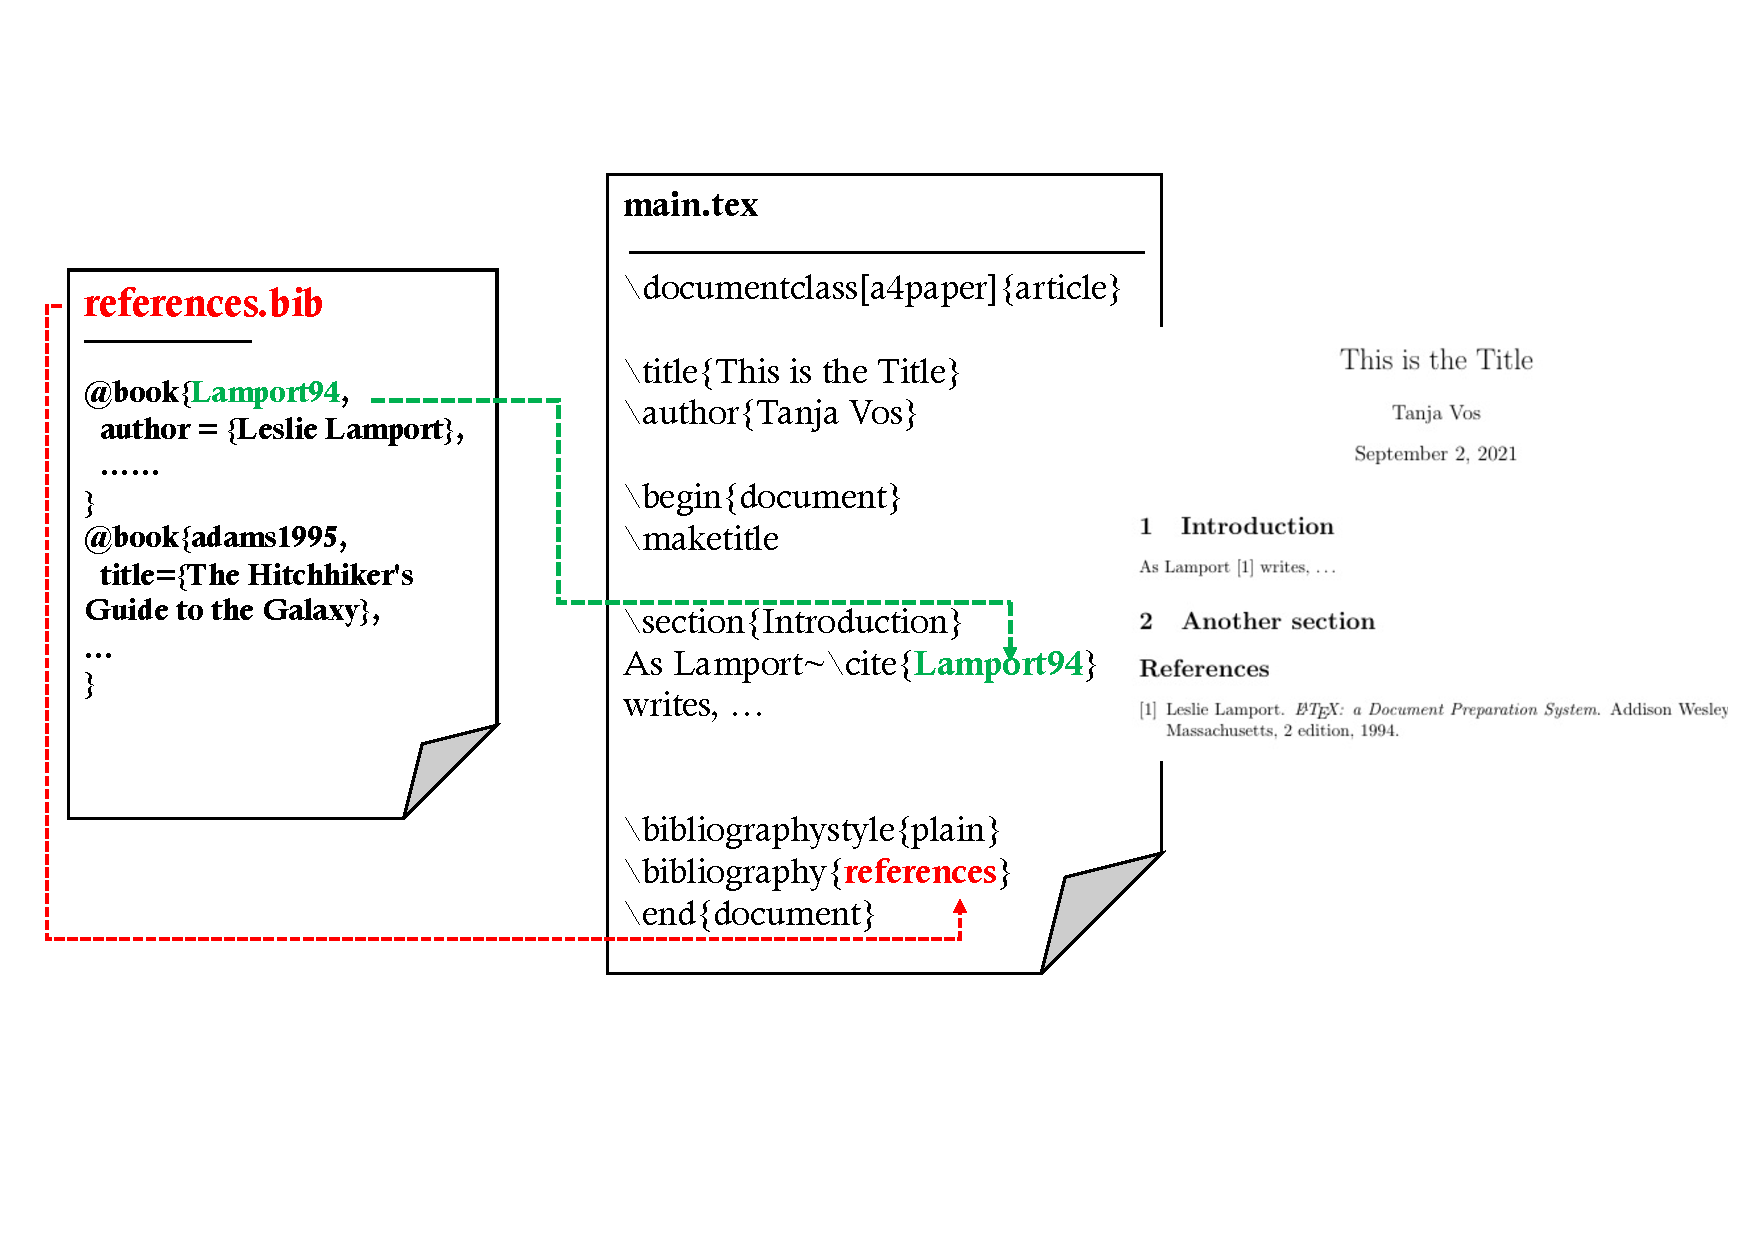
\includegraphics[scale=0.18]{images/bibentries.pdf}
\end{figure}


\end{frame}

\begin{frame}[fragile]{.bib-bestand met wetenschappelijke bronnen}

\begin{figure}
\centering
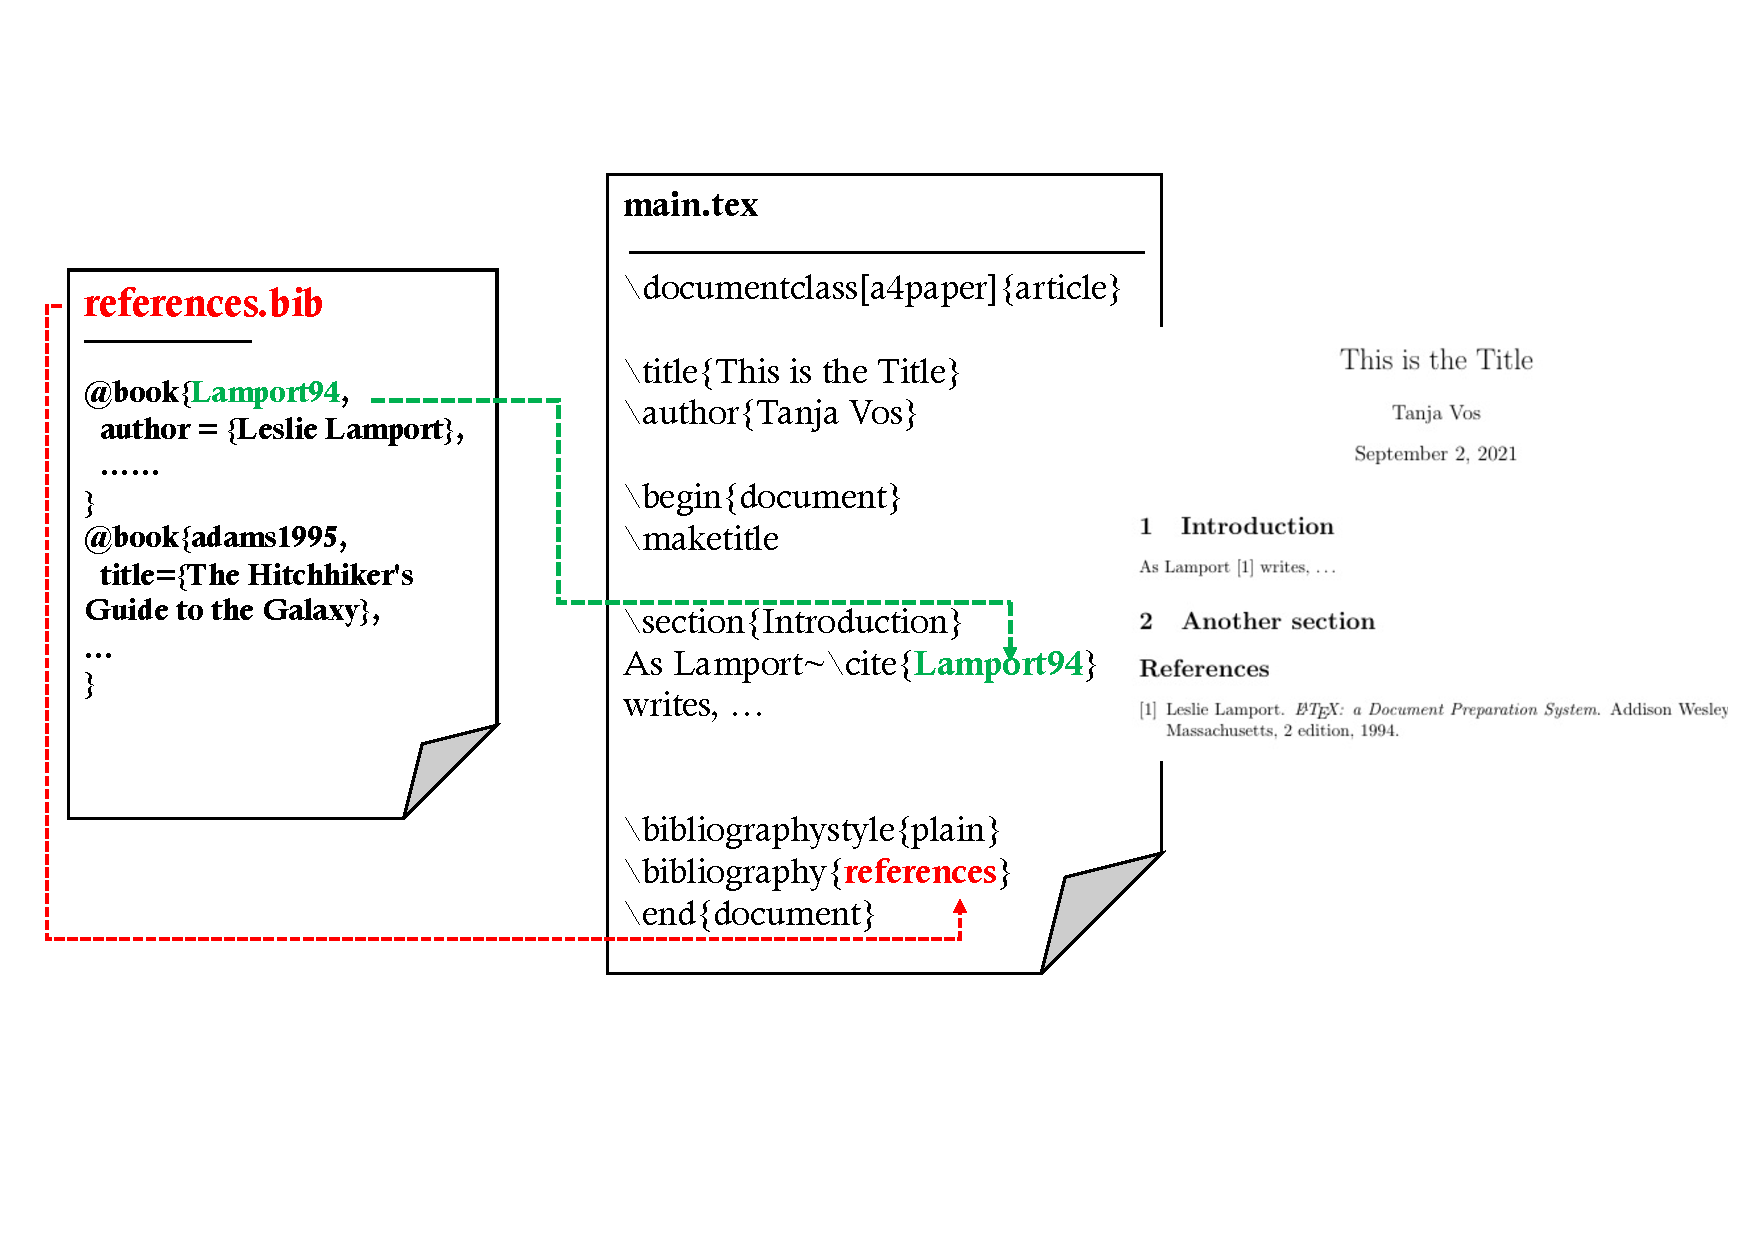
\includegraphics[scale=0.4]{images/bibentries.pdf}
\end{figure}


\small{\url{https://www.overleaf.com/read/zzvgfhsgzdky} (v3)}
\end{frame}

\section{Technische componenten in een document}
\frame[noframenumbering,plain]{\tableofcontents[currentsection, hideothersubsections, sectionstyle=show/show]}

\subsection{Wiskunde}
     
%\begin{tcolorbox}[colback=red!5!white,colframe=red!75!black,title=SOURCE]
%\end{tcolorbox}
     
%\begin{tcolorbox}[colback=green!5!white,colframe=green!75!black,title=COMPILED]
%\end{tcolorbox}

     
\begin{frame}[fragile]{Rekenen en algebra -- voorbeelden}

\begin{tcolorbox}[colback=red!5!white,colframe=red!75!black,title=SOURCE]
\begin{verbatim}
Formule $x^2 -4 = (x + 2)(x-2)$ voor alle $x$.
\end{verbatim}
\end{tcolorbox}
 

\begin{tcolorbox}[colback=green!5!white,colframe=green!75!black,title=COMPILED]
Formule $x^2 -4 = (x + 2)(x-2)$ voor alle $x$.
\end{tcolorbox}

%\medskip\pause\vspace*{0.25cm}\hline\vspace*{0.25cm}

\begin{tcolorbox}[colback=red!5!white,colframe=red!75!black,title=SOURCE]
\begin{verbatim}
Formule $$x^2 -4 = (x + 2)(x-2)$$ voor alle $x$.
\end{verbatim}
\end{tcolorbox}
 

\begin{tcolorbox}[colback=green!5!white,colframe=green!75!black,title=COMPILED]
Formule $$x^2 -4 = (x + 2)(x-2)$$ voor alle $x$.
\end{tcolorbox}

\end{frame}

\begin{frame}[fragile]{Rekenen en algebra -- voorbeelden}

\begin{tcolorbox}[colback=red!5!white,colframe=red!75!black,title=SOURCE]
\verb|$\nexists p,q\in\mathbb{Z}:\sqrt{2}=\frac{p}{q}$| 
\end{tcolorbox}

\begin{tcolorbox}[colback=green!5!white,colframe=green!75!black,title=COMPILED]
$\nexists p,q\in\mathbb{Z}:\sqrt{2}=\frac{p}{q}$
\end{tcolorbox}


\begin{tcolorbox}[colback=red!5!white,colframe=red!75!black,title=SOURCE]
\begin{verbatim}
$$\nexists p,q\in\mathbb{Z}:\sqrt{2}=\frac{p}{q}$$
\end{verbatim}
\end{tcolorbox}

\begin{tcolorbox}[colback=green!5!white,colframe=green!75!black,title=COMPILED]
$$\nexists p,q\in\mathbb{Z}:\sqrt{2}=\frac{p}{q}$$
\end{tcolorbox}
\end{frame}
     
\begin{frame}[fragile]{Linearie algebra en analyse -- voorbeelden}

\begin{tcolorbox}[colback=red!5!white,colframe=red!75!black,title=SOURCE]
\begin{minted}{latex}
$$\begin{pmatrix}
1 & 2 & 3\\
a & b & c
\end{pmatrix}$$
\end{minted}
\end{tcolorbox}

\begin{tcolorbox}[colback=green!5!white,colframe=green!75!black,title=COMPILED]
$$\begin{pmatrix}
1 & 2 & 3\\
a & b & c
\end{pmatrix}$$
\end{tcolorbox} 
\end{frame}

\begin{frame}[fragile]{Linearie algebra en analyse -- voorbeelden}

\begin{tcolorbox}[colback=red!5!white,colframe=red!75!black,title=SOURCE]
\begin{minted}{latex}
$$\sum_{n=0}^{\infty} 
\frac{f^{(n)}(a)}{n!}(x-a)^n = 
f(a) 
+ \frac{f^{\prime}(a)}{1!}(x-a) 
+ \frac{f^{\prime\prime}(a)}{2!}(x-a)^2 
+ \ldots$$
\end{minted} 
\end{tcolorbox} 

\begin{tcolorbox}[colback=green!5!white,colframe=green!75!black,title=COMPILED]
$$\sum_{n=0}^{\infty} \frac{f^{(n)}(a)}{n!}(x-a)^n=f(a)+ \frac{f^{\prime}(a)}{1!}(x-a) + \frac{f^{\prime\prime}(a)}{2!}(x-a)^2 + \ldots$$
\end{tcolorbox} 
\end{frame}
     
\begin{frame}[fragile]{Linearie algebra en analyse -- voorbeelden}

\begin{tcolorbox}[colback=red!5!white,colframe=red!75!black,title=SOURCE]
\begin{minted}{latex}
$$\int x^2 dx = \frac{x^3}{3} +c$$
\end{minted} 
\end{tcolorbox} 

\begin{tcolorbox}[colback=green!5!white,colframe=green!75!black,title=COMPILED]
$$\int x^2 dx = \frac{x^3}{3} +c$$
\end{tcolorbox}
\end{frame}

\subsection{Informatica}

\begin{frame}[fragile]{Programmeer code}

\begin{itemize}
 \item Eenvoudigste environment om code te vertonen: \texttt{verbatim}
  \begin{itemize}
   \item \verb|\begin{verbatim} ... \end{verbatim}|
   \item \verb=\verb|$\frac{2}{3}+3$|=\\
  \end{itemize}
\end{itemize}
%

\vspace*{0.3cm}

\begin{tabular}{p{5cm}p{5cm}}
\begin{tcolorbox}[colback=red!5!white,colframe=red!75!black,title=SOURCE]
\begin{minted}{latex}
\begin{verbatim}
def tel_op(a, b):
    som = a + b
    return som
\end{verbatim}
\end{minted} 
\end{tcolorbox} 
&
\begin{tcolorbox}[colback=green!5!white,colframe=green!75!black,title=COMPILED]
\begin{verbatim}
def tel_op(a, b):
    som = a + b
    return som
\end{verbatim} 
\end{tcolorbox} \\
\begin{tcolorbox}[colback=red!5!white,colframe=red!75!black,title=SOURCE]
\begin{verbatim}
\verb|$\frac{2}{3}$|
\end{verbatim} 
\end{tcolorbox}
&
\begin{tcolorbox}[colback=green!5!white,colframe=green!75!black,title=COMPILED]
\verb|$\frac{2}{3}$|
\end{tcolorbox}
\end{tabular}
\end{frame}

\begin{frame}[fragile]{We hebben de minted package al in actie gezien}

\verb|\usepackage{minted}|

\begin{tcolorbox}[colback=red!5!white,colframe=red!75!black,title=SOURCE]
\begin{small}
\begin{verbatim}
\begin{minted}{java}
for (int i = 0; i < 5; i++) {
  System.out.println(i);
}
\end{minted}
\end{verbatim}
\end{small}
\end{tcolorbox}

\begin{tcolorbox}[colback=white,colframe=green!75!black,title=COMPILED]
\begin{minted}{java}
for (int i = 0; i < 5; i++) {
  System.out.println(i);
}
\end{minted}
\end{tcolorbox}

\end{frame}

\section{Plaatjes toevoegen}

\begin{frame}[fragile]{Plaatjes toevoegen}

\begin{tcolorbox}[colback=red!5!white,colframe=red!75!black,title=SOURCE]
\begin{minted}{latex}
\usepackage{graphicx}
....
Leuk hondje 
\includegraphics[width=3cm]{hond.jpg}
\end{minted}
\end{tcolorbox}

\begin{tcolorbox}[colback=white,colframe=green!75!black,title=COMPILED]
Leuk hondje 
\includegraphics[width=3cm]{hond.jpg}
\end{tcolorbox}

\small{\url{https://www.overleaf.com/read/hxgzrgwmstjq} (v4)}

\end{frame}


\begin{frame}[fragile]{Bronnen om verder te gaan}

\begin{itemize}
 \item \url{https://en.wikibooks.org/wiki/LaTeX}
 \item \url{https://www.overleaf.com/learn/latex/Main_Page}
 \item Books: \url{https://www.latex-project.org/help/books/}
 \item Veel vragen worden op \url{https://tex.stackexchange.com/} beantwoord
 \item Tabellen converteren/maken in je browser \url{https://tableconvert.com/}
 \item Opschonen BibTeX files \url{https://flamingtempura.github.io/bibtex-tidy/}
 \item YouTube:
 \begin{itemize}
     \item \url{https://www.youtube.com/watch?v=fCzF5gDy60g&ab_channel=AcademicLesson}
 \end{itemize}
\end{itemize}

\end{frame}

\begin{frame}[fragile]{Opdracht}

Zoek een plaatje van een leuk poesje en zet hem naast het hondje.\vspace*{0.5cm}


\begin{tcolorbox}[colback=white,colframe=green!75!black,title=Resultaat moet zijn:]
Leuk hondje 
\includegraphics[width=3cm]{hond.jpg} en poesje 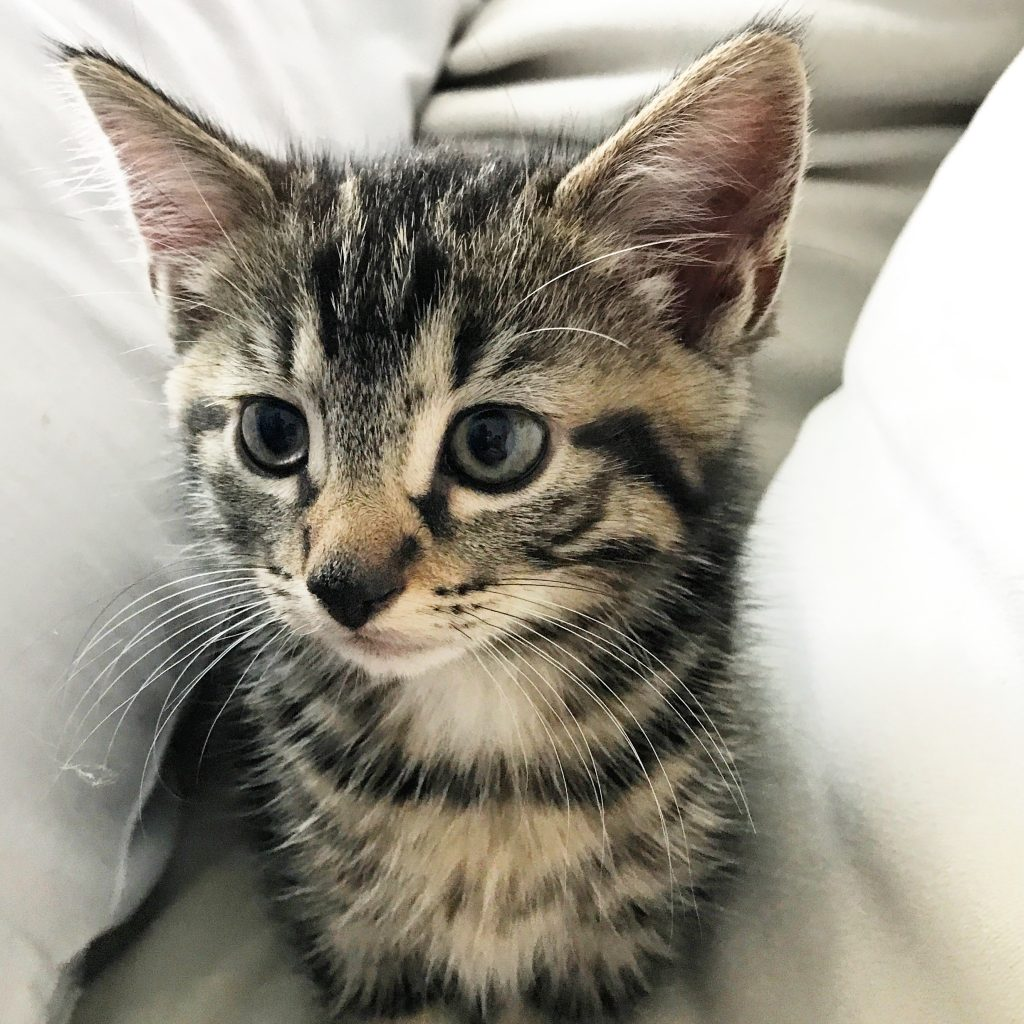
\includegraphics[width=3cm]{poes.jpg}
\end{tcolorbox}



\end{frame}

\begin{frame}[fragile]{Opdracht: Google zoeken voor oplossingen}

\begin{itemize}
\item Stel we willen niet dat onze inhoudsopgave ''Contents'' heet maar anders.

\item We willen dus de titel veranderen van onze table of contents.

\item Zoek op Google of je een oplossing van vinden voor dit probleem


\pause
\item Ik heb gezocht op: ''how can I change contents table of latex''
\item \small{\url{https://www.google.com/search?q=how+can+I+change+title+table+of+contents++latex}}
\item En ik vond een antwoord op \url{tex.stackexchange.com}
\end{itemize}

\end{frame}

\begin{frame}[fragile]{Opdracht: CTAN gebruiken}

\begin{itemize}
\item Zoek ''MusiXTEX – Sophisticated music typesetting'' op ctan

\item Browse door de documentatie en probeer het volgende toe te voegen aan je overleaf document:
\end{itemize}

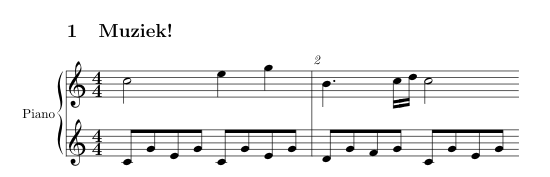
\includegraphics[width=0.8\textwidth]{images/muziek.png}


\end{frame}

\end{document}
